\subsection{Señalamiento original}

    El señalamiento original, ilustrado en la Figura \ref{fig:EJ2_2}, incluye una señal de parada próxima al final de vía absoluto (S13), señales de partida en las plataformas (S07, S09), señales de protección antes de cada paso a nivel (S11, S12), una señal de maniobras antes de converger en una vía principal (S08) y señales múltiples para cambios de vías divergentes (S11, S12, S10).
    
    \begin{figure}[H]
    	\centering
    	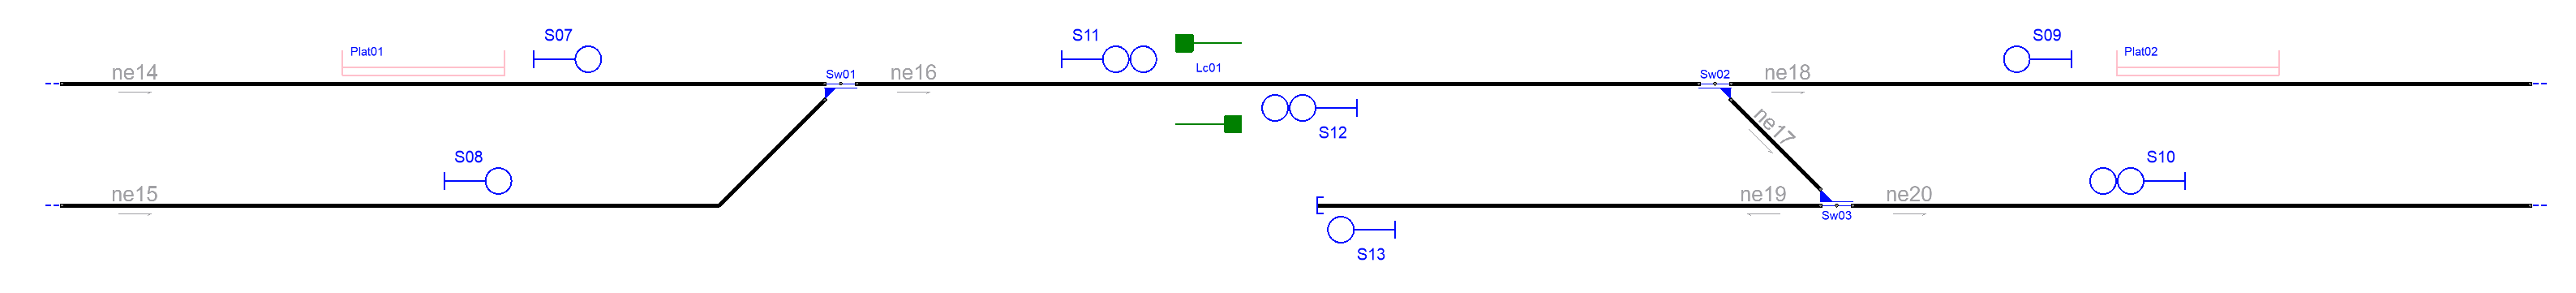
\includegraphics[width=1\textwidth]{resultados-obtenidos/ejemplo2/images/2_original.png}
    	\centering\caption{Señalamiento original del ejemplo 2.}
    	\label{fig:EJ2_2}
    \end{figure}
    
    Estas señales permiten definir hasta un máximo de 5 rutas, todas ellas detalladas en la Tabla \ref{Tab:tabla_original_2}. En una primera inspección, se puede comprobar que ninguno de los elementos ferroviarios son alcanzados por ninguna de las rutas. Además, todos los cambios de vías son utilizados, de forma simple o compuesta. 
    
    \begin{table}[H]
        {
        \caption{Tabla de enclavamiento original del ejemplo 2.}
        \label{Tab:tabla_original_2}
        \centering
        \resizebox{1\textwidth}{!}{
            \begin{tabular}{ c c c c c c c }
                \hline	
                    Ruta & Inicio & Final & Cambio & Plataforma & Cruce & netElement \\	
                \hline
                    R$_{01}$  & S$_{07}$ & S$_{11}$ & Sw$_{01}^{N}$ & - & - & ne$_{14}$-ne$_{16}$\\
                    R$_{02}$  & S$_{08}$ & S$_{11}$ & Sw$_{01}^{R}$ & - & - & ne$_{15}$-ne$_{16}$\\
                    R$_{03}$  & S$_{09}$ & S$_{12}$ & Sw$_{02}^{N}$ & - & - & ne$_{18}$-ne$_{16}$\\
                    R$_{04}$  & S$_{10}$ & S$_{13}$ & Sw$_{03}^{N}$ & - & - & ne$_{20}$-ne$_{19}$\\
                    R$_{05}$  & S$_{10}$ & S$_{12}$ & Sw$_{03}^{R}$+Sw$_{02}^{R}$ & - & - & ne$_{20}$-ne$_{17}$-ne$_{16}$\\  
                \hline
            \end{tabular}
        }
     }
    \end{table}
    
    Algunas rutas abarcan mas de un \textit{netElement}, como por ejemplo la ruta R05 que comienza en la señal S10 y finaliza en la señal S12, atravesando los \textit{netElements} ne20, ne17 y ne16, utilizando los cambios de vías Sw03 y Sw02, ambos en posición reversa.